    A criação de novos jogos de tabuleiro da UT Fábrica de Passatempos Recreativos está buscando por estagiários criativos, que possam atualizar o portfólio de produtos da empresa. Liana e Hipóleto mal entraram no programa de estágio, e já deram um abacaxi para eles resolverem.

    Por gostarem de xadrez, os recrutadores jogaram a dupla no setor de tabuleiros. Acontece que esse departamento não só está muito atrás das tendências do mundo dos jogos, como as criações elaboradas têm sido cada vez mais ``racha-cucas'', por assim dizer. Qualquer um que quiser entender o porquê, basta ver o manual do  jogo \textit{Kummirub: 2D!}, que foi apresentado para Liana e Hipóleto:

\begin{displayquote}
    \textbf{Kummirub: 2D!}

    \textit{Classificação: 10+}

    \textit{De 2 a 10 jogadores.}

    Agora o \textbf{Kummirub} virou \textbf{2D!} Em uma nova versão, este jogo irá desafiar as suas capacidades de raciocínio, e \textbf{apenas gênios poderão vencer!}
    
    \textbf{Como jogar}: Para $N$ jogadores, os números de $1$ a $N^2$ devem ser dispostos aleatoriamente nas casas do tabuleiro $N \times N$. No começo do jogo, cada jogador escolherá sua posição $i$ de $1$ a $N$. Em seguida, cada um deve escolher uma casa para cada linha do tabuleiro, totalizando $N$ casas para cada. Essas casas não poderão ser trocadas até o final da partida, e uma posição não pode pertencer a dois jogadores numa mesma rodada.

    Então, uma nova linha do tabuleiro será formada. Cada jogador deve somar os números das suas casas escolhidas, e colocar o resultado na sua posição: a $i$-ésima casa da nova linha.

    Por fim, as casas escolhidas pelos jogadores devem descer uma linha, e uma nova rodada é iniciada. Ganha o jogador que não cometer erros ao realizar as operações de cada rodada!

    Um exemplo de jogo com três jogadores pode ser visto a seguir. Para ilustrar as escolhas dos jogadores, o jogador 1 é o vermelho, o jogador 2 é o verde, e o jogador 3 é o azul:
\end{displayquote}

\begin{center}
    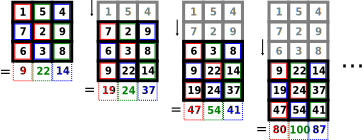
\includegraphics[scale=0.4]{kummirub/exemplo.png}
\end{center}

Liana e Hipóleto devem desenvolver uma calculadora que calcule os resultados após o $k$-ésimo turno. Você ficou responsável pelo código, e eles pelo protótipo do dispositivo, que será incluso na próxima versão do passatempo: \textit{Kummirub: 2D++!}. 

Está na hora de colocar suas habilidades de maratonista em prática! Esta primeira versão do software deverá apresentar os resultados módulo $10^9 + 7$.


\subsection*{Entrada}
A primeira linha contém o número de jogadores $N$ ($2 \leq N \leq 10$).

As próximas $N$ linhas correspondem ao tabuleiro. Cada linha contém $N$ números $C_{x, y}$ ($1 \leq C_{x, y} \leq N^2$, $0 \leq x, y < N$), o número na casa de posição ($x, y$).

A linha seguinte contém o número do turno $T$ ($1 \leq T \leq 10^8$).

Por fim, as $N$ linhas seguintes são referentes às casas escolhidas pelos jogadores. Cada linha contém $N$ números $i_{x, y}$ ($1 \leq i \leq N$), o número do jogador que escolheu a posição ($x, y$).


\subsection*{Saída}
Imprima uma linha com $N$ números $r_i$: o resultado do jogador $i$ após $T$ turnos, em módulo $10^9 + 7$.

Não coloque um espaço após o último resultado, apenas uma nova linha (`\textbackslash n').


%----- Exemplo 1 -----%
%\newpage
\begin{table}[!h]
\centering
\begin{tabular}{|l|l|}
\hline
\begin{minipage}[t]{3in}
\textbf{Exemplo de entrada}
\begin{verbatim}
3
1 5 4
7 2 9
4 3 8
4
1 2 3
3 1 2
1 3 2
\end{verbatim}
\vspace{1mm}
\end{minipage}
&
\begin{minipage}[t]{3in}
\textbf{Exemplo de saída}
\begin{verbatim}
74 96 83
\end{verbatim}
\vspace{1mm}
\end{minipage} \\
\hline
\end{tabular}
\end{table}

%----- Exemplo 2 -----%
\begin{table}[!h]
\centering
\begin{tabular}{|l|l|}
\hline
\begin{minipage}[t]{3in}
\textbf{Exemplo de entrada}
\begin{verbatim}
2
1 2
3 4
10000
2 1
1 2
\end{verbatim}
\vspace{1mm}
\end{minipage}
&
\begin{minipage}[t]{3in}
\textbf{Exemplo de saída}
\begin{verbatim}
492026538 492026538
\end{verbatim}
\vspace{1mm}
\end{minipage} \\
\hline
\end{tabular}
\end{table}
